\documentclass[a4paper,10pt]{article}
 
\usepackage[T1]{fontenc}
\usepackage[utf8]{inputenc}
\usepackage{textcomp}
\usepackage[T1]{fontenc}
\usepackage{graphicx}
\usepackage{xcolor, colortbl}
\usepackage{caption}
\usepackage{listings}
\usepackage{wrapfig} 
\usepackage{tabu} % For coloring single row of table
\usepackage{scrextend}
%\usepackage{hyperref}

\renewcommand\familydefault{\sfdefault} 
\usepackage{tgheros}
\usepackage[defaultmono]{droidmono}

\usepackage{amsmath,amssymb,amsthm,textcomp}
\usepackage{enumerate}
\usepackage{multicol}
\usepackage{tikz}

\usepackage{geometry}
\usepackage{trace}
\usepackage{tcolorbox}
\usepackage{tabularx}
\usepackage{accsupp}% http://ctan.org/pkg/accsupp


\tcbuselibrary{listings,skins} % For lstlisting

\geometry{total={210mm,297mm},
left=25mm,right=25mm,%
bindingoffset=0mm, top=20mm,bottom=20mm}


% For coloring single row in table
\def\zapcolorreset{\let\reset@color\relax\ignorespaces}
\def\colorrows#1{\noalign{\aftergroup\zapcolorreset#1}\ignorespaces}

\newcommand{\linia}{\rule{\linewidth}{0.5pt}}
\newcommand{\ano}{\text{2}}

% custom theorems if needed
\newtheoremstyle{mytheor}
    {1ex}{1ex}{\normalfont}{0pt}{\scshape}{.}{1ex}
    {{\thmname{#1 }}{\thmnumber{#2}}{\thmnote{ (#3)}}}

\theoremstyle{mytheor}
\newtheorem{defi}{Definition}

%%% Declare title %%%%%%%%%%%%%%%%%%%%%%%%%%%%%%%%%%%%%%%%%%%%%%%%
\newcommand{\antitle}{\text{Verilog Modelling Techniques}}
% my own titles
\makeatletter
\renewcommand{\maketitle}{
\begin{center}
\vspace{2ex}
{\huge \textsc{{{\large}Assignment - \ano}\vspace{0.1cm} \break \antitle}}
\vspace{1ex}
\\
%%%%%%%%%%%%%%%%%%%%%%%%%%%%%%%%%%%%%%%%%%%%%%%%%%%%%%%%%%%%%%%%%%

Department of Electronics and Communication Engineering \\
Indian Institute of Technology, Roorkee
\linia\\
ECN 104 \hfill Digital Logic Design
\vspace{4ex}
\end{center}
}
\makeatother
%%%

% custom footers and headers
\usepackage{fancyhdr}
\pagestyle{fancy}
\lhead{}
\chead{}
\rhead{}
\lfoot{Assignment \ano\ - \antitle}
\cfoot{}
\rfoot{Page \thepage}
\renewcommand{\headrulewidth}{0pt}
\renewcommand{\footrulewidth}{0pt}
%

\definecolor{vgreen}{RGB}{104,180,104}
\definecolor{vblue}{RGB}{49,49,255}
\definecolor{vorange}{RGB}{255,143,102}

\makeatletter
\newcommand*\@lbracket{[}
\newcommand*\@rbracket{]}
\newcommand*\@colon{:}
\newcommand*\colorIndex{%
    \edef\@temp{\the\lst@token}%
    \ifx\@temp\@lbracket \color{black}%
    \else\ifx\@temp\@rbracket \color{black}%
    \else\ifx\@temp\@colon \color{black}%
    \else \color{vorange}%
    \fi\fi\fi
}
\makeatother

\definecolor{codebg}{RGB}{250,250,240} 
\definecolor{greatblue}{RGB}{91,155,215} 

% Set up caption and labels for lstlistings
\DeclareCaptionFont{white}{\color{white}}
\DeclareCaptionFormat{listing}{\colorbox{greatblue}{\parbox{\textwidth}{\hspace{1cm}#1#2#3}}}
\captionsetup[lstlisting]{format=listing,labelfont=white,textfont=white}

\renewcommand{\thelstnumber}{% Line number printing mechanism
  \protect\BeginAccSupp{ActualText={}}\arabic{lstnumber}\protect\EndAccSupp{}%
}

\def\backtick{\char18} 
\lstdefinestyle{verilog-style}
{
    %columns=fullflexible, 
    language=Verilog,
    basicstyle=\small\ttfamily,
    keywordstyle=\color{vblue},
    identifierstyle=\color{black},
    commentstyle=\color{vgreen},
    numbers=left, 
    numberstyle=\color{gray},  
    numbersep=10pt,
    moredelim=*[s][\colorIndex]{[}{]},
    literate=*{:}{:}1, 
%    backgroundcolor=\color{codebg},
%    framexrightmargin=0.09cm, 
    framexleftmargin=-0.09cm,
    frame=trbl,
    upquote=true, 
    framerule=0pt,
    keepspaces=true
}

\lstdefinestyle{verilog-inline-style}
{
    language=Verilog,
    basicstyle=\small\ttfamily,
    keywordstyle=\color{vblue},
    identifierstyle=\color{black},
    commentstyle=\color{vgreen},
    moredelim=*[s][\colorIndex]{[}{]},
    literate=*{:}{:}1, 
    upquote=true, 
    framerule=0pt,
    keepspaces=true
}

\newcommand{
  \insertverilog}[3]{
  \lstinputlisting[label=#2, caption=#3, style={verilog-style}]{#1}
}


% Command for problem
\newcounter{problemNumber}
\setcounter{problemNumber}{1}
\newcommand {
  \insertProblem}[1]{
  \vspace{0.5cm}
  \hrule
  \vspace{0.3cm}

  {\color{greatblue}\textbf{\large{Problem \theproblemNumber}}}
  \vspace{2pt}\\#1

  \addtocounter{problemNumber}{1}
  \vspace{0.2cm}
  \hrule  
  \vspace{0.5cm}
}


%%%----------%%%----------%%%----------%%%----------%%%
% Command for creating a resource box
\newcommand{\resourcebox}[2]{
  \fbox{%
    \parbox{0.5\textwidth}{%
      \text{#1}
    }%
  } 
}


%%%----------%%%----------%%%----------%%%----------%%%

\makeatletter
\def\lst@outputspace{{\ifx\lst@bkgcolor\empty\color{white}\else\lst@bkgcolor\fi\lst@visiblespace}}
\makeatother


%%%----------%%%----------%%%----------%%%----------%%%
\begin{document}

\title{Assignment \ano \\ Modelling Sequential Logic Using Verilog}

\maketitle
\tableofcontents
\section{Introduction}
Verilog supports wide variety of modelling techniques. Different
modelling techniques allows hardware description at different level of
abstraction, starting from switch level modelling (PMOS/NMOS) and all
the way up to behavioural modelling (algorithmic description). Each
one of them have their own benefits and use cases. In this assignment
we will discuss three of them, namely Gate-level modelling, structural
modelling and behavioural modelling.

\subsection{Gate-level modelling}
Gate-level modelling in Verilog is used to describe a circuit only
using logic gates. This approach is used to describe critical parts of
a design, like adders and multipliers. Using gate-level implementation
allows greater control over the design than other
techniques. Gate-level modelling is only used for small scale design,
due to its complexity other modelling techniques are commonly used to
abstract gate level implementation.

\subsubsection{Gate Primitives in Verilog}
Verilog support following gates:
\begin{multicols}{2}
  \begin{itemize}
  \item AND
  \item NAND
  \item OR
  \item NOR
  \item XOR
  \item XNOR
  \item NOT
  \end{itemize}
\end{multicols}


Gates in Verilog are available as primitives and can be instantiated
similar to modules, Listing \ref{gate-level-impl} is an example gate
level circuit.

\insertverilog{./verilog_files/gateLevelExample.v}{gate-level-impl}{\text{Example module using Gate-level modelling}}

Verilog also supports instantiating gates without a instance name
demonstrated in Listing \ref{gate-instance-without-name}.
\insertverilog{./verilog_files/unnamedGate.v}{gate-instance-without-name}{\text{Instantiating unnamed gates}}

\subsubsection{Delay specification}
All the circuits we have studied so far have no delay associated with
them, these are called 0-delay circuits. Real circuits however, always
have a delay between their input and output. Verilog allows modelling
of delays at various level of abstraction using delay statements.

Syntax for specifying a delay is:
\begin{lstlisting}[style=verilog-inline-style, xleftmargin=0.2\textwidth]
  <gate_primitive> #(<delay>) <inst_name>(...ports...) 
\end{lstlisting}

For example:
\begin{lstlisting}[style=verilog-inline-style, xleftmargin=0.25\textwidth]
  /* 2-input AND gate with 1 time unit delay */
  and #(1) a1(result, input1, input2);
\end{lstlisting}

\vspace{0.1cm}
To specify unit of delay we'll write a compiler
directive, this is typically written at the begining of the
description.

\begin{center}
  \begin{lstlisting}[style=verilog-inline-style,xleftmargin=.35\textwidth]
    `timescale 1ns/1ps
  \end{lstlisting}
\end{center}


Here \lstinline[upquote=true]{1ns} is the time unit while
\lstinline[upquote=true]{1ps} is the time resolution. Which will be
explained in later assignment. A complete example using delay
statements is given in Listing \ref{delay-example}.

\insertverilog{./verilog_files/delayExample.v}{delay-example}{\text{Example usage of delays statement to specify propagation delay of logic gates.}}

\insertProblem { NOT gate is one of the primitives available with
  Verilog, NOT gate is a type of buffer and is also known as inverting
  buffer. Buffers in digital circuit is often used to isolate two
  parts of a circuit, but this isolation can also be added with a
  certain behaviour like inversion of signal or delaying signal to
  synchronize with other parts.
  
  \begin {enumerate}
  \item Write a Verilog module which acts as an inverting buffer (NOT
    gate), you have to use verilog primitive
    \lstinline[style=verilog_inline_style]{not} for the
    implementation, use the testbench
    \textsc{testbench{\ano}.{\theproblemNumber}.1.v} for testing your
    design.
  \item Another kind of buffer often used in digital circuit is the
    `non-inverting buffer'. As the name suggests, the non-inverting
    buffer doesn't invert the input. This buffer seems to be of no use
    since it cannot do any processing. This leads us to its one of the
    common use case, using buffer to level translation. Level
    translation is used whenever two parts of a circuit are powered
    with different Vdd. Now that you know what a buffer is, write a
    Verilog module to implement a buffer using the inverting buffers
    you designed in Problem {\theproblemNumber}.1.
  \item NOT gates are also used in ring oscillators, which is a kind
    of an oscillator often used to generate clock signals. Ring
    oscillator is an oscillator which looks like a ring, and contains
    a chain of odd number of NOT gates. Ring oscillator's frequency
    depends on the delay of the NOT gate and number of gates used. A
    simple 3 NOT gate ring oscillator is shown in
    Fig. \ref{ring-oscillator}. Let the propagation delay of each of
    the gate in \Fig. \ref{ring-oscillator} be $t_d$, intuitively one
    can say that the delay between change of values at point is
    $3t_d$. Use this information and calculate the time period of an n
    NOT gate ring oscillator, where n is an odd number.

    \begin{figure}[!h] \centering  
      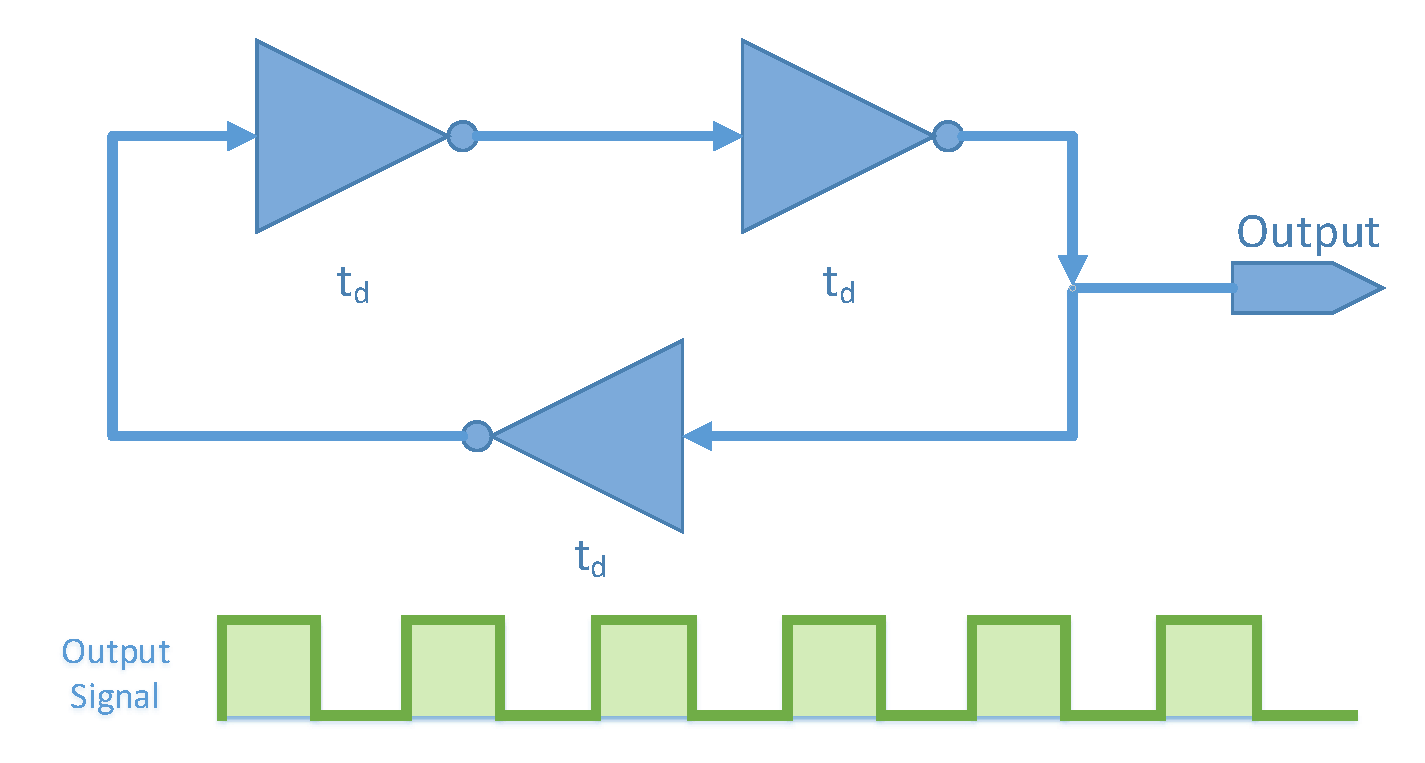
\includegraphics[width=0.5\linewidth]{./resources/ringOscillator.pdf}
      \caption{Simulation result for Listing \ref{ring-oscillator}, output changes 15ns after the change in input.} 
      \label{ring-oscillator}
    \end{figure}

  \item Using the expression from the Problem {\theproblemNumber}.3,
    write the description of a module for a 5 NOT gate ring
    oscillator. You have to design the ring oscillator such that the
    time period of the generated wave should be 30ns, assume that each
    of the NOT gate has a propagation delay of 5ns. Use
    \textsc{testbench{\ano}.{\theproblemNumber}.4.v} to test your
    design.

  \item Using the expression from the Problem {\theproblemNumber}.3,
    write the description of a module for a 5 NOT gate ring
    oscillator. You have to design the ring oscillator such that the
    time period of the generated wave should be 30ns, assume that each
    of the NOT gate has a propagation delay of 5ns. Use
    \textsc{testbench{\ano}.{\theproblemNumber}.4.v} to test your
    design.
  \item Will a single not gate ring oscillator work? Why?
  \end{enumerate}
} 


\subsection{Data-flow Modelling}
%https://stackoverflow.com/questions/28751979/difference-between-behavioral-and-dataflow-in-verilog#28759581
Data flow modelling is a higher level of abstraction. Describing a
circuit using data-flow modelling does not require knowledge of gates
level circuit, thus it is easier than gate-level modelling when
description of large scale circuits are written.  All the examples
from Assignment 1 used data flow modelling.

\subsubsection{Continuous Assignment}
\label{continuous-assignment}
Continuous assignment in Verilog are used for data flow modelling,
these assignment starts with
\lstinline[style=verilog-inline-style]{assign} keyword. Continuous
assignment drives value into a net
(\lstinline[style=verilog-inline-style]{wire}). Following example
describes use of continuous assignment:

{\color{red}\textbf{Note:}} Verilog is concurrent language unlike
programming languages such as C,C++ or Java. All the continuous
assignments are evaluated at the same time.

\insertverilog{./verilog_files/continuousAssignment.v}{continuous-assignment}{Example usage of continuous assignment.}

Continuous assigment in Verilog can also be done implicitly, which
assigning value on declaration of a net
(\lstinline[style=verilog-inline-style]{wire}). Implicit delcaration
of Verilog is down as follows:
\begin{lstlisting}[style=verilog-inline-style,xleftmargin=.25\textwidth]
  wire new_wire = input1 & input2;
\end{lstlisting}

\subsubsection{Assignment Delays}
Similar to gate-level modelling, Verilog allows specifying delays in
assignment to model real circuits. Assignment delay specify the delay
between the change of LHS and RHS of a continuous assignment. Listing
\ref{assignment-delay} shows example usage of assignment delay while
Fig. \ref{assignment-delay-sim} shows simulation result of Listing
\ref{assignment-delay}.

\insertverilog{./verilog_files/assignmentDelay.v}{assignment-delay}{Using assignment delay in Verilog.}

\begin{figure}[!h] \centering  
  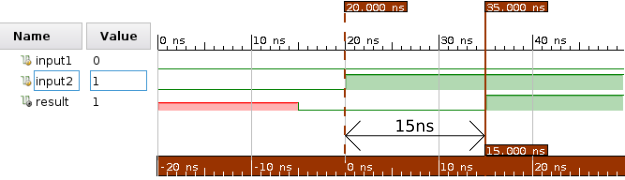
\includegraphics[width=0.8\linewidth]{./resources/assignmentDelay.png}
  \caption{Simulation result for Listing \ref{assignment-delay}, output changes 15ns after the change in input.} 
  \label{assignment-delay-sim}
\end{figure}

\pagebreak
\insertProblem {
  Multiplexer is a digital element which is used to select a single signal from a group of signals. Block diagram of a multiplexer is shown in Fig. \ref{multiplexer}, the input $\text{in}_1$ and $\text{in}_2$ are multiplexed and the output is decided using the input $\text{c}$. If the input c is 0 then $\text{output}=\text{in}_1$ else $\text{output}=\text{in}_2$.
  
  \begin{figure}[!h] \centering  
    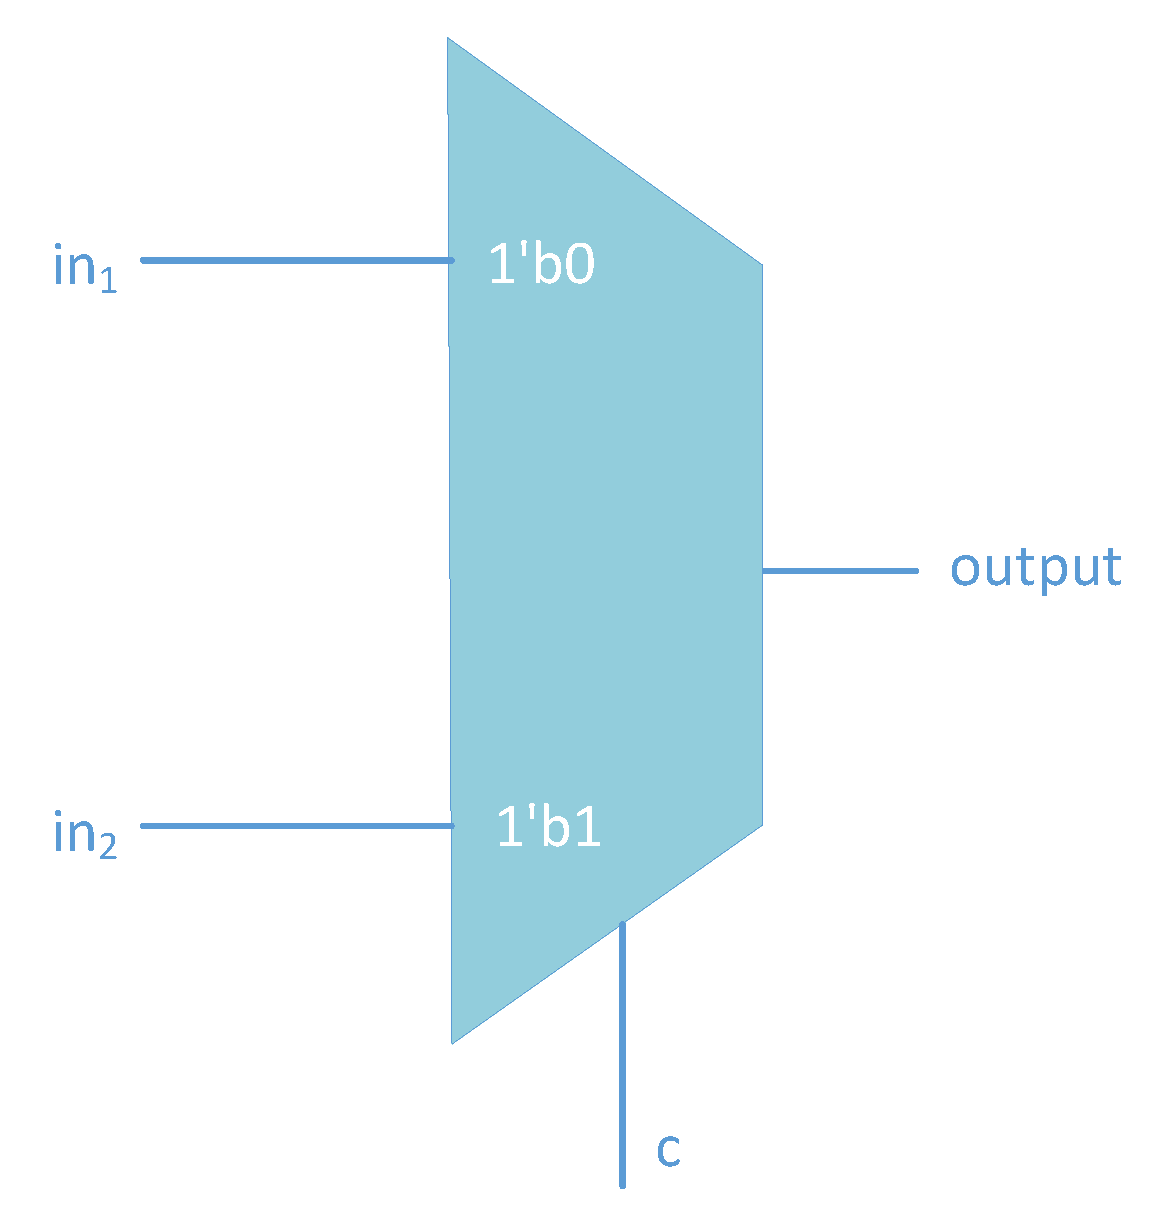
\includegraphics[width=0.3\linewidth]{./resources/multiplexer.pdf} 
    \caption{Simulation result for Listing \ref{assignment-delay}, output changes 15ns after the change in input.} 
    \label{multiplexer} 
  \end{figure}

  \begin{enumerate}
    
  \item Write the hardware description of a 2-to-1 multiplexer using
    Verilog, you have to implement this using only behaviourial
    modelling. (\textit{Hint: Verilog supports the Ternary operator,
      which has same behaviour as in programming languages.})
  \item To verify the behaviour of multiplexer you just described,
    write a testbench to test its behaviour. The testbench should
    generate all different permutations of the inputs. To keep things
    simple, you can for now verify the behaviour using waveform
    viewer.
  \item Now suppose you want to model a multiplexer you just purchased
    from the market, which has a prpogation delay of 2ns. Modify the
    module from part 1 such that the behaviour of your description
    matches the one you bought.  }
\section{Behavioral Modelling}
Behavioral modelling is a higher level of modelling where circuit
description is written as its behaviour, this algorithmic
representation of a circuit abstracts the details of gate-level and
data flow modelling. Behavioral modelling resembles more to
programming languages such as C than circuit description.


\subsection{\lstinline[style=verilog-inline-style]{reg} Element}
\lstinline[style=verilog-inline-style]{reg} element is used to
represent abstract storage device in
Verilog. \lstinline[style=verilog-inline-style]{reg}s can be used to
store information (single bit or of arbitrary length using
vector). We'll get back to usage of
\lstinline[style=verilog-inline-style]{reg} and will differentiate it
with \lstinline[style=verilog-inline-style]{wire} after studying
procedural blocks.

\subsection{Procedural Blocks}
Earlier we read about continuous assignment which allows us to drive
value to a net whenever the driver changes, this kind of assignment
allows only to describe combinational circuit. To describe sequential
circuits Verilog provides procedural blocks, these blocks are used to
drive values to net (\lstinline[style=verilog-inline-style]{reg}) only
inf the condition is met.

\subsection{\lstinline[style=verilog-inline-style]{initial} Block}
\lstinline[style=verilog-inline-style]{Initial} blocks in Verilog are
used to specify initial values of all the storage elements. When
simulation starts simulator doesn't know what values are to be
assigned to storage elements. Initial block begins with
\lstinline[style=verilog-inline-style]{initial begin} and ends with
\lstinline[style=verilog-inline-style]{end}. Initial blocks gets
executed only once when the simulation is started.

{\color{red}\textbf{Note:}} Only a
\lstinline[style=verilog-inline-style]{reg} can be assigned values
inside an \lstinline[style=verilog-inline-style]{initial} block, this
is because unlike \lstinline[style=verilog-inline-style]{wire} which
are used for connection \lstinline[style=verilog-inline-style]{reg}
stores information and this information is unknown to the simulator at
t=0. Structure of an initial block is given in Listing \ref{initial-structure}.

\insertverilog{./verilog_files/initialStructure.v}{initial-structure}{Structure of an initial block.} 

\subsection{\lstinline[style=verilog-inline-style]{always@} block}
\lstinline[style=verilog-inline-style]{always@} block in Verilog are
used for describing a event which should happen only under certain
conditions, such as change in value of one of the elements.
 
Basic structure of an \lstinline[style=verilog-inline-style]{always@}
block is given in Listing \ref{always-structure}.

\insertverilog{./verilog_files/alwaysStructure.v}{always-structure}{Structure of an always@ block.} 

Listing \ref{always-example} shows a module which changes output only
one the positive edge of input
\lstinline[style=verilog-inline-style]{clk}. 

\insertverilog{./verilog_files/alwaysExample.v}{always-example}{Synchronous logic which changes value of result only at the positive edge of clk.} 
 
\subsection{Blocking and Non-Blocking Assignment}
\subsubsection{Blocking Assignments}
Blocking assingments are assignments which block the simulation while
their value is being calculated. This means that theexecution flow
will stop at this statement until it is executed. Blocking assignment in Verilog is done using \lstinline[style=verilog-inline-style]{=}. Listing \ref{non-working-blocking-assignment} demonstrates the functioning of blocking assignment.

\insertverilog{./verilog_files/nonWorkingSwap.v}{non-working-blocking-assignment}{Swapping bytes using blocking assignment.}  

In the above example (Listing \ref{non-working-blocking-assignment})
statement 18 doesn't gets executed until statement 17 is executed,
this is due to the use of blocking assignment.

\subsubsection{Non-blocking Assignments} 
In Listing \ref{non-working-blocking-assignment} we saw that blocking
assignments cannot be used to swap bytes, this is where non-blocking
assignments will come to use. Non-blocking assignments are evaluated
in two steps first all the RHS values are calculated at the begining
of the procedural block, and then the value is assigned to LHS when
the execution reaches particular statement.

Listing \ref{working-swap} shows how non-blocking assignments can be
used for swapping bytes.

\insertverilog{./verilog_files/workingSwap.v}{working-swap}{Swapping bytes using non-blocking assignment\, it works!}   

\section{Differences between \lstinline[style=verilog-inline-style]{wire} and \lstinline[style=verilog-inline-style]{reg} and where to use what}
\subsection{Legal use of \lstinline[style=verilog-inline-style]{wire}}
Wires in Verilog are used to connect two elements, they can be assigned a value or a value can be read from them. However they cannot store it, you'll have to drive them with values (constant, other wires or regs).

\begin{itemize}
\item \lstinline[style=verilog-inline-style]{wire}s are allowed only in continuous assignments (page \pageref{continuous-assignment}).
\item A \lstinline[style=verilog-inline-style]{wire} cannot be assigned a value inside a procedural block.
\item \lstinline[style=verilog-inline-style]{wire} can be used to assign a value to a \lstinline[style=verilog-inline-style]{reg} or a \lstinline[style=verilog-inline-style]{wire}.
\end{itemize}

\subsection{Legal use of \lstinline[style=verilog-inline-style]{reg}}
\lstinline[style=verilog-inline-style]{reg}s in Verilog are storage elements, they however do not represent physical registers. Once synthesized they can be represented by a physical register, RAM or ROM.

 \begin{itemize}
 \item \lstinline[style=verilog-inline-style]{reg}s cannot be assigned a value using continuous assigment.
 \item A \lstinline[style=verilog-inline-style]{wire} can only be assigned a value in a procedural block.
 \item \lstinline[style=verilog-inline-style]{wire} can be used to assign a value to a \lstinline[style=verilog-inline-style]{reg} or a \lstinline[style=verilog-inline-style]{wire}.
\end{itemize}

\subsection{Places where both \lstinline[style=verilog-inline-style]{wire} and \lstinline[style=verilog-inline-style]{reg} are allowed}

\pagebreak
\section*{References}
\begin{itemize}
  \small 
% https://electronics.stackexchange.com/questions/29553/how-are-verilog-always-statements-implemented-in-hardware
\item http://inst.eecs.berkeley.edu/{\textasciitilde}cs150/fa08/Documents/Always.pdf
\item Aenean in sem ac leo mollis blandit.  
\end{itemize}

\section*{Additional resources}
\begin{itemize}
  \small 
\item Stack Exchange: How are Verilog “always” statements implemented in hardware? \\\textit{http://bit.ly/verilogAlwaysStatement}
\item Stack Overflow: Difference between behavioral and dataflow in verilog \\\textit{http://bit.ly/modellingDiff}
\item Stack Overflow: How can I know if my code is synthesizable? [Verilog] \\\textit{http://bit.ly/synthCode}
\end{itemize} 

\centerline{\textit{These resources are great for expanding your understanding, but...}}
\begin{centering}
  \begin{figure}[!h] \centering  
    
\includegraphics[width=0.5\linewidth]{./resources/meme.jpeg} 
  \end{figure}  
\end{centering}

\end{document}

